% !TeX spellcheck = en_GB
% !TeX encoding = UTF-8
% !TeX root = ../thesis.tex
\chapter{Background}\label{chap:background}
%TODO Unfinished chapter!

As this thesis merges known concepts from \scratch{} analysis and \ngram{}, we introduce the concepts our work is based on in the following sections. Section~\ref{sec:analysing-scratch} introduces \scratch{} and its functionality as a block-based programming language as well as the \scratch{} analyser \litterbox{}. Section~\ref{sec:language-models} introduces the concept of a \ngram{}. It is necessary to understand the difference between n-grams and a n-gram model and the way of using it in order to obtain valuable information about \scratch{} code.


\section{Analysing \scratch{} Programs}\label{sec:analysing-scratch}
The functionality of \scratch{} is important to understand in order to follow the main research of this thesis. The following methods and analysis is based on the programming language \scratch{} itself and \litterbox{} which is the basis of the evaluation and used its \AST{} as a guideline for the structure of the n-gram model. 

\subsection{The Structure of \scratch{}}\label{subsec:scratch}
\scratch{}\footnote{\url{https://en.scratch-wiki.info/wiki/Scratch}, last accessed August 19, 2020} is a block-based programming language designed for kids that was created by the \textit{Massachusetts Institute of Technology}\footnote{\url{https://web.mit.edu/}, last accessed September 06, 2020}. With over 50 million registered users and shared projects\footnote{\url{https://scratch.mit.edu/statistics/}, last accessed August 19, 2020} it is one of the most popular tools for teaching children from a young age how to develop computational thinking skills to solve problems programmatically.

The 'drag-and-drop-programming' style that \scratch{} is utilizing allows the programmer to pick from a pallet of existing blocks and build scripts by combining these code pieces like a jigsaw puzzle.
\textit{Blocks}\footnote{\url{https://en.scratch-wiki.info/wiki/Blocks}, last accessed August 19, 2020} are separated into different types that include \textit{hat, stack, reporter, boolean and cap}. Each data type has a specific shape that indicates their intended usage in order to avoid errors in the syntax of the code. In contrast to text-based programming languages, the \textit{blocks} help children to memorize the commands and avoid structure errors that otherwise would very likely occur in the beginning. 

After combining different \textit{blocks}, \textit{scripts}\footnote{\url{https://en.scratch-wiki.info/wiki/Script}, last accessed August 19, 2020} are created which resemble code methods in \java{}. \textit{Scripts} are found in the code of the actors that perform the actions, called \textit{sprites}\footnote{\url{https://en.scratch-wiki.info/wiki/Sprite}, last accessed August 19, 2020} as well as the \textit{stage}\footnote{\url{https://en.scratch-wiki.info/wiki/Stage}, last accessed August 19, 2020} which visualises the background of the created program. 

Figure~\ref{fig:scratchblocks} shows the typical structure of a \scratch{} \textit{script} that uses most of the before mentioned data types. Starting the \textit{script} with a \textit{hat} and ending with a \textit{cap} block, there are also 10 different categories that each block is assigned to: \textit{Motion, Looks, Sound, Event, Control, Sensing, Operators, Variables, List, and My Blocks}. 

\begin{figure}[t]
    \centering
    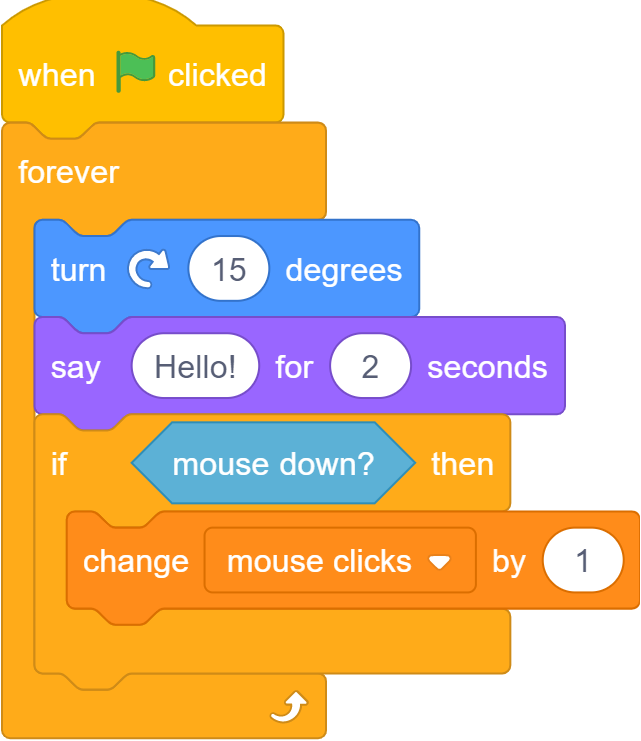
\includegraphics[scale=0.4]{scratchblocks.png}
    \caption[A representative \scratch\ script]{\label{fig:scratchblocks} A representative script in scratch.}
\end{figure}

For instance, the Figure~\ref{fig:script} of a \scratch{} project that is based on the band BTS\footnote{\url{https://scratch.mit.edu/projects/308718195/}, last accessed August 20, 2020} shows a \textit{script} that controls the picture of one of the band members which is shown in Figure~\ref{fig:sprite}. Once the user clicks on the profile picture of Jungkook, the 'click' event of the \textit{script} is fired and the text "Saranghae <3" is shown for 2 seconds.

\begin{figure}[t]
    \centering
    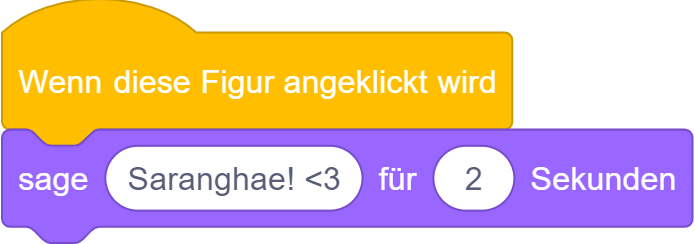
\includegraphics[scale=0.4]{jungkook_script.png}
    \caption[Program that controls a sprite]{\label{fig:script} A \scratch{} script controlling a corresponding sprite}
\end{figure}

\begin{figure}%
    \centering
    \subfloat[Sprite in front of a background]{{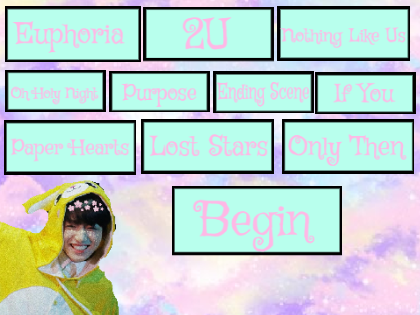
\includegraphics[width=7cm]{jungkook_stage.png} }}%
    \qquad
    \subfloat[Sprite responding to the clicked event]{{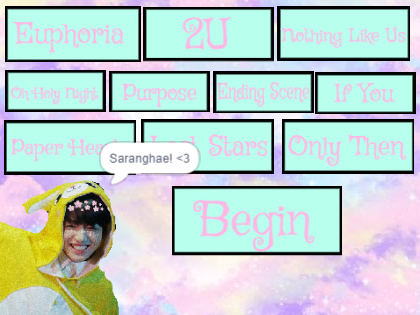
\includegraphics[width=7cm]{jungkook_stage_action.png} }}%
    \caption[A sprite's reaction after an executed event]{\label{fig:sprite}A \scratch{} stage and sprite that respond to events}%
\end{figure}

\subsection{The Static \scratch{} Code Analyser \litterbox{}}\label{subsec:litterbox}
\litterbox{}\footnote{\url{https://gitlab.infosun.fim.uni-passau.de/se2/litterbox}, last accessed August 19, 2020} is a static code analysis tool for detecting bugs in \scratch{} projects where \scratch{} code is saved as a JSON file and downloaded, for example using the \scratch{} REST API\footnote{\url{https://projects.scratch.mit.edu}, last accessed August 20, 2020}. \litterbox{} then creates an abstract syntax tree (AST) for a \scratch{} project. The occurrence of bugs in code is mostly the consequence of recurring bad code writing habits. With the help of \litterbox{} these bug patterns and code smells can be filtered and analysed in order to correct the found bugs and avoid similar mistakes in the future. \litterbox{} is developed at the Chair of Software Engineering II and the Didactics of Informatics of the University of Passau and is the foundation for the analysis of \scratch{} programs with n-gram models in this bachelor's thesis. 


\section{N-gram Language Model}\label{sec:language-models}
Statistical language models, in its essence, are the type of models that assign probabilities to the sequences of words. The \ngram{} is the simplest model that assigns probabilities to sentences and sequences of words. You can think of an N-gram as the sequence of N words. A 2-gram or bigram is a two-word sequence of words like 'please read', 'read very', or 'very carefully', and a 3-gram or trigram is a three-word sequence of words like 'please read very', or 'read very carefully'. 

\subsection{Probability Calculation of N-grams}\label{subsec:ngram}
\ngram{} usually consists of sentences \textit{s} of words \textit{w} that are all based on a specific dictionary {D}. Using \hyperref[def:markov_chain]{Markov chains} the language model calculates a  probabilistic distribution of all possible sequences that can occur in the language based on \textit{D}.

\begin{definition}[Markov chain]\label{def:markov_chain}
    %
    ``A usually discrete stochastic process (such as a random walk) in which the probabilities of occurrence of various future states depend only on the present state of the system or on the immediately preceding state and not on the path by which the present state was achieved''~\cite{markov_chain}
    %
\end{definition} 

The probability of \textit{s} is then calculated by partitioning it into its individual words \textit{w}. But the probability of \textit{w} is only dependent on the n-1 previous words. Given a sentence \( s = w_1w_2w_3\cdots w_m \) the probability is estimated with the Formula ~\ref{eq:ngram-prob} where \(h_i = w_{1-n}\cdots w_i \) is the history sequence for the conditional probability of \(w_i\):

\begin{equation} \label{eq:ngram-prob}
P(x) ={} \displaystyle\prod_{i=1}^{m} P(w_i|h_{i-1})
\end{equation}

For instance, in the case of a 3-gram each word is dependent on the probability of the last \(n - 1 = 3 - 1 = 2 \) words. Therefore the probability of the sentence s = 'Would you like to go outside?' can be estimated with the Formula~\ref{eq:trigram-prob}:

\begin{equation}\label{eq:trigram-prob}
\begin{aligned}
P(s) ={} & P(Would)\cdot P(you|Would)\cdot P(like|Would\ you) \\ 
		 & \cdot P(to|you\ like)\cdot P(go|like\ to)\cdot P(outside|to\ go)
\end{aligned}
\end{equation} 
  
\subsection{N-gram Model Configuration}\label{subsec:configuration}
%TODO Explain n-gram model
There are five key factors that affect the amount of bugs that a language model can find. These are the important \textit{configuration parameters} that need to be set in order to achieve optimal results:  

\begin{definition}[Gram Size]\label{def:gram_size}
    %
    ``The size of a n-gram model. Different gram sizes enable the model to use different internal probabilities to calculate the probabilities of \hyperref[def:token]{token} sequences.''~\cite{bugram}
    %
\end{definition}
The \hyperref[def:gram_size]{gram size n} is an essential part of building a \ngram{} and calculating the probabilities of a token sequence by utilizing n-1 predecessors. Existing studies found that 3 to 6-gram models gave the best results, although the optimal \textit{gram size} for bug detection is still unknown. To explore this question more, Section \ref{sec:gram_size} focuses on analysing the effects of different gram sizes in the \scratch{} bug detection as one of the research questions of this bachelor's thesis.

\begin{definition}[Sequence Length]\label{def:sequence_length}
    %
    ``The length of token sequences to be considered when building n-gram models and detecting bugs. Different sequence lengths enable the model to capture different program scenarios and further affect the performance of the bug detection.''~\cite{bugram}
    %
\end{definition}

The \hyperref[def:sequence_length]{length} of analysed sequences of a project is essential to get a detailed analysis of the project structure. The amounts of code blocks and scripts in a \scratch{} project can vary from 1 to a few hundred. By breaking the program into smaller parts, more bugs can be obtained.

\begin{definition}[Reporting Size]\label{def:reporting_size}
    %
    ``The number of sequences, in the bottom of the ranked list, which will be reported as bugs. An appropriate number may reduce the amount of false positives.''~\cite{bugram}
    %
\end{definition}

In contrast to the usual rule-based bug finding techniques which use a probability threshold to distinguish potential bugs from normal sequences, the \ngram{} detects token sequences of low absolute probabilities. The goal is to find the optimal parameter for the \hyperref[def:reporting_size]{reporting size} that separates buggy sequences from false positives. A larger amount of bugs that get reported from the found list, will definitely lead to a bigger size of found bugs but also means a higher risk of reporting sequences that are normal occurrences.

\begin{definition}[Minimum Token Occurrence]\label{def:minimum_token_occurrence}
    %
    ``The minimum number of times a token must occur in the code to be included in an n-gram model. An appropriate value helps to filter out \hyperref[def:token]{token} sequences that use unusual/special methods, thus have low probabilities but are not bugs.''~\cite{bugram}
    %
\end{definition}

Taking out tokens in a project that are not frequently used by manifesting a \hyperref[def:minimum_token_occurrence]{minimum token occurrence} is common practice for natural language processing (NLP) techniques. It reduces the chances of falsely reporting uncommon token sequences that are not bugs but just very uncommonly used. 

\begin{definition}[Probability Threshold]\label{def:probability_threshold}
    %
    ``If a \hyperref[def:token]{token} sequence does not reach this probability threshold, it can be considered a bug or unusual occurrence.''
    %
\end{definition}

After the analysis of a project a number of sequences with the least calculated probabilities are getting reported as bugs. But in order to minimize the amount of false positives in the bug set, it is common practice to determine a \hyperref[def:probability_threshold]{probability threshold} that differentiates a bug from a rare occurrence of a sequence. 